\section*{Testfunktionen}

Quadratische Funktion
\[
| x - x_d |^2
\]

Exponentielle Funktion
\[
e^{|x|^2}
\]
\begin{figure}[h]
  \centering
  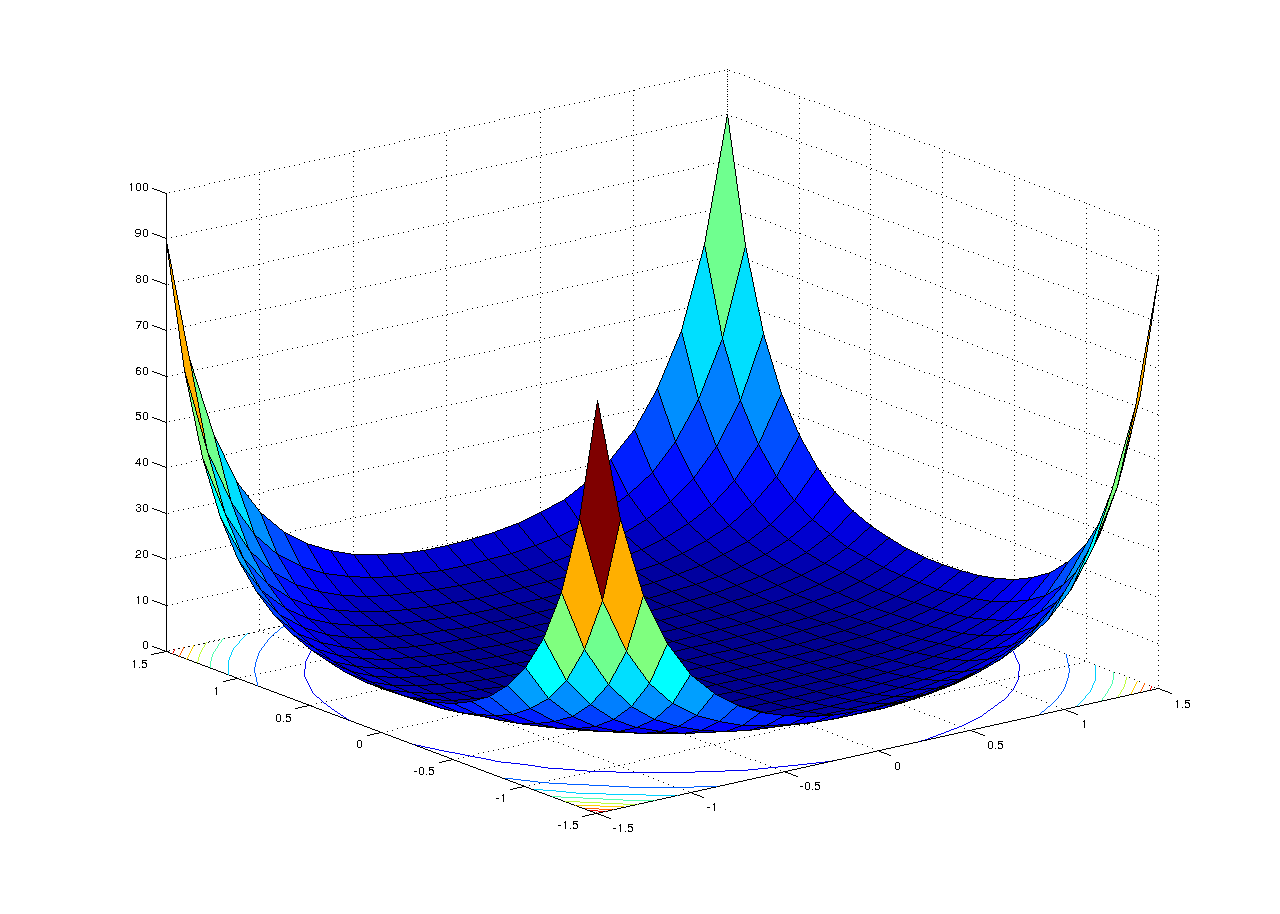
\includegraphics[width=0.75\textwidth]{exp-func}
  \caption{Exponentielle Funktion}
  \label{fig:exp_func}
\end{figure}

Rosenbrock Funktion
\[
100(x_2-x_1^2)^2+(1-x_1)^2
\]
\begin{figure}[h]
  \centering
  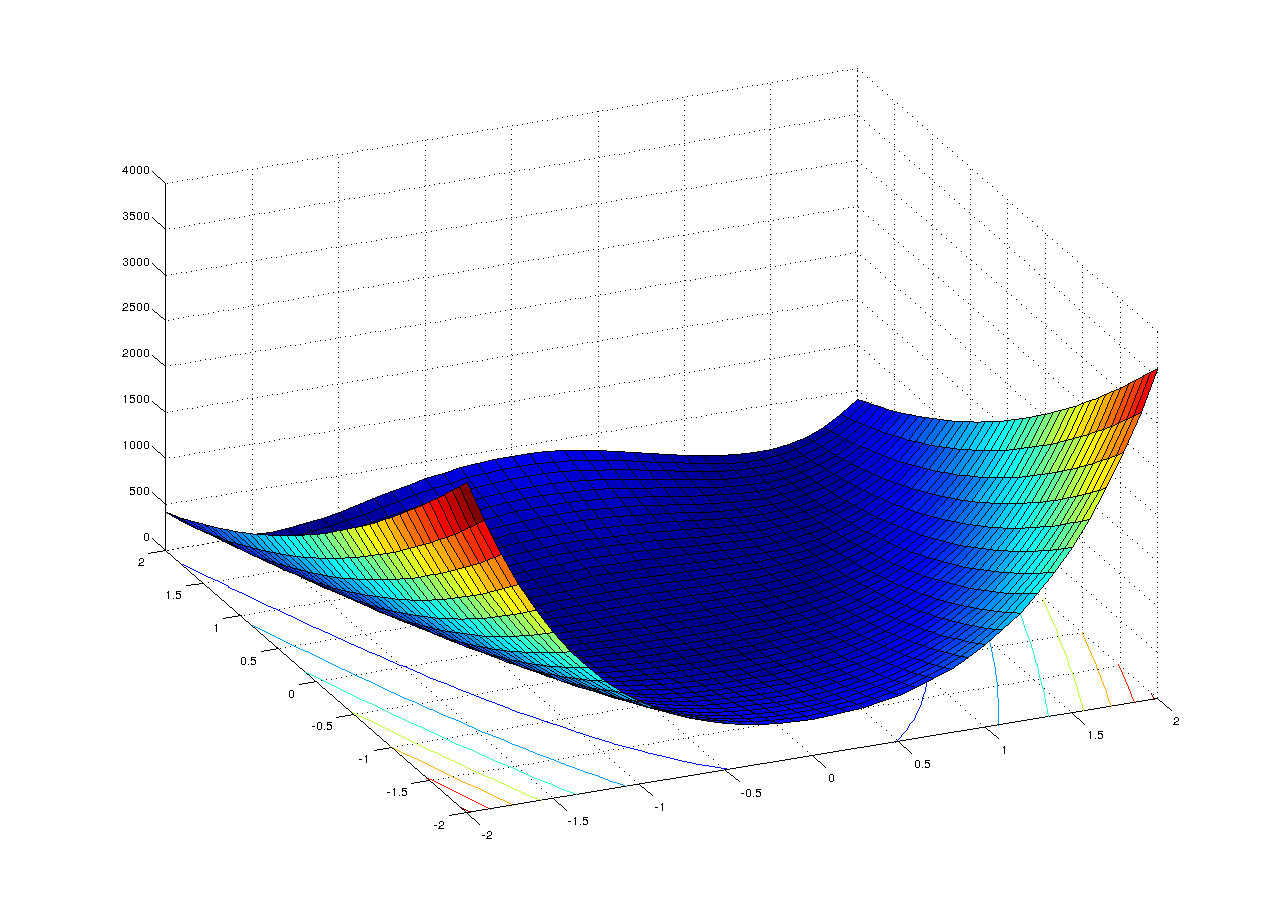
\includegraphics[width=0.75\textwidth]{rosenbrock}
  \caption{Rosenbrock Funktion}
  \label{fig:rosenbrock}
\end{figure}

Himmelblau Funktion
\[
(x_1^2+x_2-11)^2 + (x_1+x_2^2-7)^2
\]
\begin{figure}[h]
  \centering
  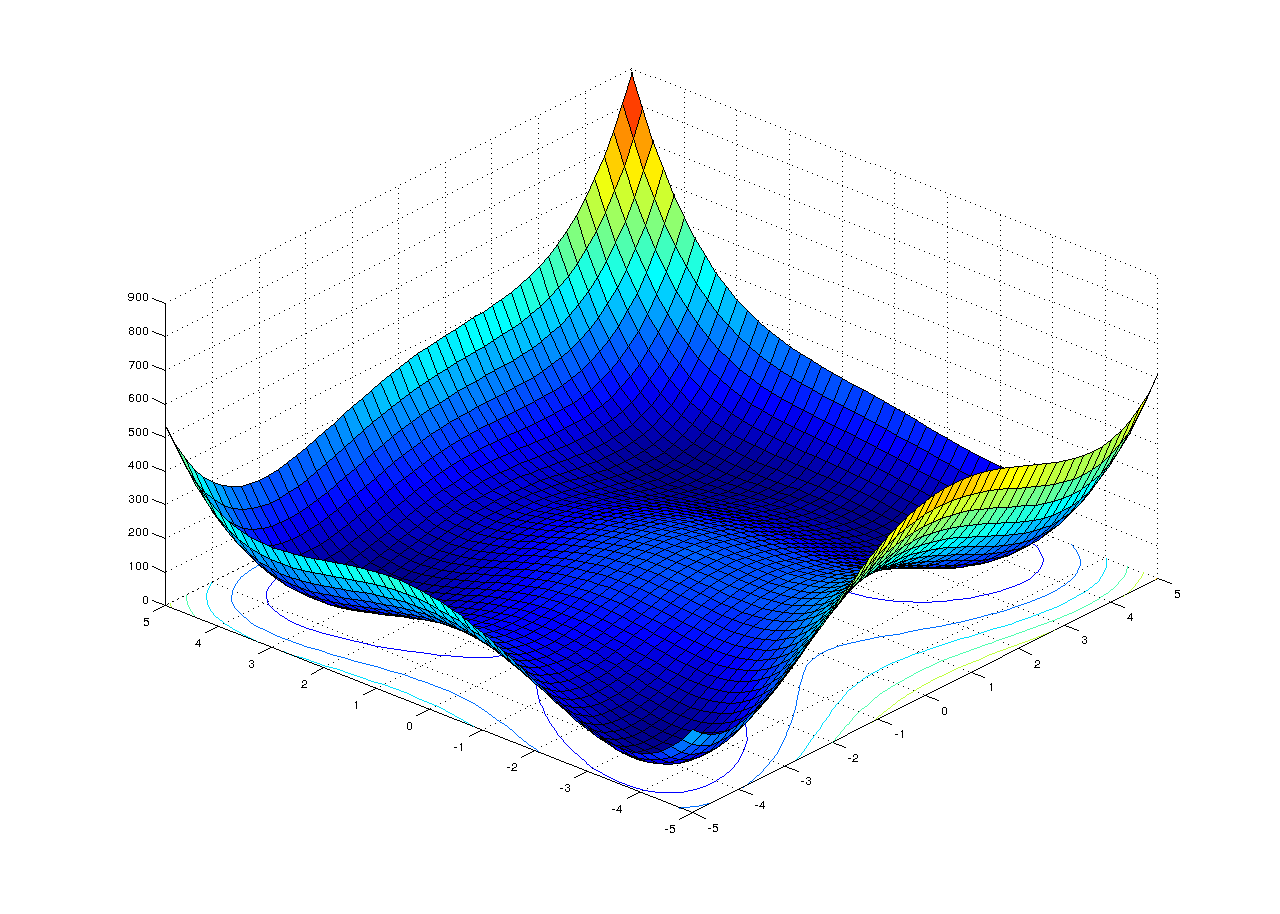
\includegraphics[width=0.75\textwidth]{himmelblau}
  \caption{Himmelblau Funktion}
  \label{fig:himmelblau}
\end{figure}

Bazaraa-Shetty Funktion
\[
(x_1-2)^4+(x_1-2x_2)^2
\]
\begin{figure}[h]
  \centering
  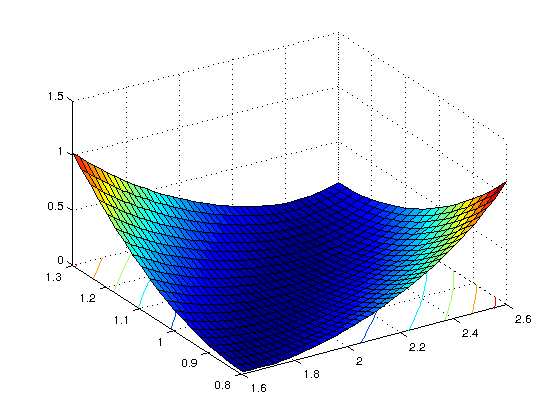
\includegraphics[width=0.75\textwidth]{bazaraa-shetty}
  \caption{Bazaraa-Shetty Funktion}
  \label{fig:bazaraa_shetty}
\end{figure}

Schuldt Funktion
\[
x_2+10^{-5}(x_2-x_1^2)^2
\]

Asaadi Funktion
\[
x_2+\frac{1}{3}(x_1+1)^3
\]

McCormick Funktion
\[
\sin(x_1+x_2) + (x_1-x_2)^2 - 1.5x_1 + 2.5x_2 + 1
\]

Dixon Funktion
\[
(1-x_1)^2 + \sum_{k=1}^{9} (x_k^2-x_{k+1})^2 + (1-x_{10})^2
\]

Colville Funktion
\[
100(x_2-x_1^2)^2 + (1-x_1)^2 + 90(x_4-x_3^2)^2 + (1-x_3)^2
+ 10.1((x_2-1)^2 + (x_4-1)^2) + 19.8(x_2-1)(x_4-1)
\]

Betts Funktion
\[
2 - \frac{1}{2}x_1x_2
\]

Paviani Funktion
\[
- (\ln(x_1-2))^2 - (\ln(10-x_1))^2
- (\ln(x_2-2))^2 - (\ln(10-x_2))^2
\]